\documentclass{article}

\usepackage{minitoc}
\usepackage{tabularx}
\usepackage{booktabs}
\usepackage{graphicx}
\usepackage{hyperref}
\usepackage{xcolor}
\usepackage{blkarray}
\usepackage{amsthm, amssymb, amsmath}
\usepackage{caption}
\usepackage{subcaption}
\usepackage{multirow}
\usepackage{multicol}
\usepackage[ruled,vlined]{algorithm2e}

\usepackage{natbib}
\bibliographystyle{abbrvnat}

\theoremstyle{definition}
\newtheorem{definition}{Definition}[section]
\newtheorem{theorem}{Theorem}[section]
\newtheorem{lemma}[theorem]{Lemma}
\newtheorem{conjecture}[theorem]{Conjecture}
\newtheorem{Prop}{Proposition}

\usepackage[margin=2.5cm, includefoot, footskip=30pt]{geometry}
\pagestyle{plain}
\setlength{\parindent}{0em}
\setlength{\parskip}{1em}

\renewcommand{\baselinestretch}{1}

\usepackage{standalone}

\newtheorem{proposition}{Proposition}

\title{Reactive strategies with longer memory}

\author{Nikoleta E. Glynatsi, Ethan Akin, Martin Nowak, Christian Hilbe}
\date{}

\begin{document}

\maketitle

\section{Formal Model}

We consider infinitely repeated games among two players, player $p$ and
player $q$. Each round, they engage in the donation game with payoff matrix

\begin{equation} \label{Eq:DonationGame}
\left(
\begin{array}{cc}
b-c	&-c\\
b	&0
\end{array}
\right).
\end{equation}

Here $b$ and $c$ denote the benefit and the cost of cooperation, respectively. 
We assume $b\!>\!c\!>\!0$ throughout.
Therefore, the payoff matrix~\eqref{Eq:DonationGame} is a special case of the
prisoner's dilemma with payoff matrix,

\begin{equation} \label{Eq:PrisonerDilemma}
    \left(
    \begin{array}{cc}
    R & S\\
    T & P
    \end{array}
    \right),
\end{equation}

with $T > R > S > P$ and $2 R > T + S$. Here, $R$ is the reward payoff of mutual
cooperation, $T$ is the temptation to defect payoff, $S$ is the sucker's payoff,
and $P$ is the punishment payoff for mutual defection.

We assume in the following, that the players' decisions only depend on the
outcome of the previous $n$ rounds. To this end, an {\it $n$-history for player
$p$} is a string $h^p=(a^p_{-1},\ldots,a^p_{-n})\!\in\!\{C,D\}^n$. An entry
$a^p_{-k}$ corresponds to player $p$'s action $k$ rounds ago. Let $H^p$ denote
the space of all $n$-histories of player~$p$. Analogously, let $H^q$ as the set
of $n$-histories $h^q$ of player~$q$. Sets $H^p$ and $H^q$ contain
$|H^p|=|H^q|=2^{n}$ elements each.

A pair $h\!=\!(h^p,h^q)$ is called an {\it $n$-history of the game}. We use
$H=H^p\times H^q$ to denote the space of all such histories. This set contains
$|H|=2^{2n}$ elements.

{\bf Memory-$n$ strategies.} A {\it memory-$n$} strategy is a vector
$\mathbf{m}=(m_h)_{h\in H}\in[0,1]^{2n}$. Each entry $m_h$ corresponds to the
player's cooperation probability in the next round, depending on the outcome of
the previous $n$ rounds. If the two players use memory-$n$ strategies
$\mathbf{m}$ and $\mathbf{m'}$, one can represent the interaction as a Markov
chain with a $2^{2n}\!\times\!2^{2n}$ transition matrix $M$. Let
$\mathbf{v}=(v_h)_{h\in H}$ be an invariant distribution of this Markov chain.
Based on the invariant distribution $\mathbf{v}$, we can also compute the
players' payoffs. To this end, let $\mathbf{S}^k = (S_h^k)_{h\in H}$ denote the
vector that returns for each $h$ the one-shot payoff that player $p$ obtained
$k$ rounds ago,

\begin{equation}
    S_h^k = \left\{
    \begin{array}{cl}
    b-c	&\text{if}~ a_{-k}^p=C~\text{and}~ a_{-k}^q=C\\
    -c	&\text{if}~ a_{-k}^p=C~\text{and}~ a_{-k}^q=D\\
    b	&\text{if}~ a_{-k}^p=D~\text{and}~ a_{-k}^q=C\\
    0	&\text{if}~ a_{-k}^p=D~\text{and}~ a_{-k}^q=D
    \end{array}
    \right.
\end{equation}

Then we can define player $p$'s repeated-game payoff $s_{\mathbf{m},\mathbf{m'}}$ as

\begin{equation} \label{Eq:Payoff}
s_{\mathbf{m},\mathbf{m'}}  = \mathbf{v}\cdot \mathbf{S}^1 = \mathbf{v}\cdot \mathbf{S}^2 = \ldots = \mathbf{v} \cdot \mathbf{S}^n.
\end{equation}

The equalities $\mathbf{v}\cdot \mathbf{S}^1 = \ldots = \mathbf{v} \cdot
\mathbf{S}^n$ correspond to the intuition that it does not matter which of the
past $n$ rounds we use to define average payoffs. The payoff
$s_{\mathbf{m'},\mathbf{m}}$ of player $q$ can be defined analogously.

Let's provide definitions for some additional terms that will be used in this
manuscript.

{\bf Nash Strategies.} A strategy $\mathbf{m}$ for player $p$, is a \textit{Nash
strategy}, if player $q$ never receives a payoff higher than that of the mutual
cooperation payoff. Irrespective of $q$'s strategy. Namely if,

\begin{equation}\label{Eq:Nash}
    s_{\mathbf{m'},\mathbf{m}} \leq (b - c) \; \forall \; m'.
\end{equation}

{\bf Nice Strategies.} A player's strategy is \textit{nice}, if the player is
never the first to defect.

{\bf Partner Strategies.} For player $p$, a \textit{partner strategy} is a nice
strategy such that,

\begin{align}\label{Eq:Partner}
    s_{\mathbf{m'},\mathbf{m}} & < (b - c) \; \Rightarrow \; s_{\mathbf{m},\mathbf{m'}} < (b - c), ~~and~~\\
    s_{\mathbf{m'},\mathbf{m}} & \geq (b - c) \; \Rightarrow \; s_{\mathbf{m'},\mathbf{m}} = s_{\mathbf{m},\mathbf{m'}} = (b - c).
\end{align}

irrespective of the co-player's strategy. In other words, partners strive to
achieve the mutual cooperation payoff R with their co-player. However, if the
co-player doesn't cooperate, they are prepared to penalize them with lower
payoffs. Partner strategies, by definition, are best responses to themselves,
making them Nash strategies~\cite{Hilbe:GEB:2015}. All partner strategies are
Nash strategies, but not all Nash strategies are partner strategies.

{\bf \%ToDo} Why are partner strategies interesting to study?

Previously the work, of \citep{akin:EGADS:2016} characterized all partner
strategies for $n=1$. For higher memory ($n>1$) a few
works~\citep{hilbe:PNAS:2017} have managed to characterized partner strategies
bit only a subset of them because as memory increases analytical results become
more difficult to obtain. However, in this work we characterize all partner
reactive strategies for $n=2, n=3$. We formally introduce reactive strategies
and present the results from section \ref{section:reactive_strategies} onwards.
In the next section, we will discuss a series of results for the general case of
memory$-n$.

\section{An Extension of Akin's Lemma}

The work of~\citep{akin:EGADS:2016} focuses on the case of memory-one
strategies, thus for $n=1$. A memory-one strategy of player $p$ is the vector
$\mathbf{m} = (m_1, m_2, m_3, ,m_4)$, and against a co-player $\mathbf{m}'$ the
stationary distribution is of $\mathbf{v} = (v_1, v_2, v_3, v_4)$. Akin's lemma
states the following,

\begin{lemma}[Akin's Lemma]\label{lemma:akin}

Assume that player \(p\) uses the memory-one strategy \(\mathbf{m}=(m_1, m_2,
m_3, m_4)\), and \(q\) uses a strategy that leads to a sequence of distributions
\(\{\mathbf{v}^{(n)}, n = 1, 2, ...\}\) with \(\mathbf{v}^{(k)}\) representing
the distribution over the states in the \(k^{\text{th}}\) round of the game. Let
\(\mathbf{v}\) be the associated stationary distribution, and let
\(\mathbf{\tilde{m}} = \mathbf{m} - \mathbf{e}_{12}\) where \(\mathbf{e}_{12} =
(1, 1, 0, 0)\). Then,
  
    \begin{align}
      \lim_{n \rightarrow \infty} \frac{1}{n} \sum_{k=1}^{n} \mathbf{v}^{(k)} \cdot \mathbf{\tilde{m}} & = 0, \text{ and therefore } \mathbf{v} \cdot \mathbf{\tilde{m}} = 0. \\
      \mathbf{v} \cdot \mathbf{\tilde{m}} = (m_{CC} - 1) v_{CC} + & (m_{CD} - 1) v_{CD} + m_{DC} v_{DC} + m_{DD} v_{DD}.
    \end{align}
\end{lemma}

The interpretation of this lemma is that the player's probabilities $p$ of
switching from cooperation to defection and from defection to cooperation are
equal. This is due to the fact that player $p$ can only switch from cooperation
to defection if they have previously switched from defection to cooperation.

In the following we generalise Akin's Lemma to $n>1$. Before we do so, we provide
some further, definition.

One special case of such a memory-$n$ strategy is the  {\it round-$k$-repeat
strategy}. Player $p$ uses a {\it round-$k$-repeat strategy}
$\mathbf{m}^{k-\text{Rep}}$ if in any given round, the player chooses the same
action as $k$ rounds ago. That is, if the game's $n$-history is such that
$a^p_{-k}\!=\!C$, then $m^{k-\text{Rep}}_h\!=\!1$; otherwise
$m^{k-\text{Rep}}_h\!=\!0$.

With the same method as in \citep{akin:EGADS:2016}, one can show {\it Akin's
Lemma}: For each $k$ with $1\!\le\!k\!\le\!n$, the invariant distribution
$\mathbf{v}$ satisfies the following relationship,

\begin{equation} \label{Eq:AkinsLemma}
\mathbf{v} \cdot (\mathbf{m}-\mathbf{m}^{k-\text{Rep}}) \!=\! \sum_{h\in H} v_h (m_h-m_h^{k-\text{Rep}}) = 0.
\end{equation}

The intuition for this result is that $\mathbf{v}\cdot \mathbf{m}$ and all
$\mathbf{v}\cdot \mathbf{m}^{k-\text{Rep}}$ are just different (but equivalent)
expressions for player $p$'s average cooperation rate. For example,
$\mathbf{v}\cdot\mathbf{m}$ corresponds to a setup in which one first draws a
history $h$ according to the invariant distribution $\mathbf{v}$; then one takes
player $p$'s probability $m_h$ to cooperate in the next round; the expectation
of this procedure is $\sum_{h\in H} v_h m_h$.

\noindent
{\bf Zero-determinant strategies.}
Based on Akin's Lemma, we can derive a theory of zero-determinant strategies
analogous to the case of memory-one strategies. In the following, we say a
memory-$n$ strategy $\mathbf{m}$ is a zero-determinant strategy if there are
$k_1$, $k_2$, $k_3$ and $\alpha$, $\beta$, $\gamma$ such that $\mathbf{m}$ can
be written as

\begin{equation} \label{Eq:DefZD}
\mathbf{m} = \alpha \mathbf{S}^{k_1} + \beta \mathbf{\tilde{S}}^{k_2} + \gamma \mathbf{1} + \mathbf{m}^{k-\text{Rep}},  
\end{equation} 
where $\mathbf{1}$ is the vector for which every entry is 1. By Akin's Lemma and the definition of payoffs,
\begin{equation} \label{Eq:PayoffZD}
0 = \mathbf{v} \cdot  (\mathbf{m} - \mathbf{m}^{k-\text{Rep}}) = \mathbf{v} \cdot (\alpha \mathbf{S}^{k_1} + \beta \mathbf{\tilde{S}}^{k_2} + \gamma \mathbf{1} ) = \alpha s_{\mathbf{m}, \mathbf{m'}} + \beta s_{\mathbf{m'}, \mathbf{m}} + \gamma. 
\end{equation}

That is, payoffs satisfy a linear relationship. 

One interesting special case arises if $k_1\!=\!k_2\!=\!k_3\!=:\!k$ and $\alpha
= -\beta =1/(b\!+\!c)$ and $\gamma=0$. In that case, the formula
\eqref{Eq:DefZD} yields the strategy

\begin{equation}
m_h = \left\{
\begin{array}{ll}
1	&\text{if}~~a^q_{-k}=C\\
0	&\text{if}~~a^q_{-k}=D
\end{array}
\right.
\end{equation}

That is, this strategy implements Tit-for-Tat (for $k\!=\!1$) or delayed
versions thereof (for $k\!>\!1$). By Eq.~\eqref{Eq:PayoffZD}, the enforced
payoff relationship is $s_\mathbf{p}\!=\! s_\mathbf{q}$ (in particular, these
strategies are {\it partners}).

Another interesting special case arises if  $k_1\!=\!k_2\!=\!k_3\!=:\!k$ and
$\alpha\!=\!0$, $\beta\!=\!-1/b$, $\gamma\!=\!1\!-\!c/b$. In that case
Eq.~\eqref{Eq:DefZD} yields the strategy

\begin{equation}
m_h = \left\{
\begin{array}{ll}
1	&\text{if}~~a^q_{-k}=C\\
1-c/b	&\text{if}~~a^q_{-k}=D
\end{array}
\right.
\end{equation}

That is, the generated strategy is GTFT (if $k\!=\!1$), or delayed versions
thereof (for $k\!>\!1$). By Eq.~\eqref{Eq:PayoffZD}, the enforced payoff
relationship is $s_{\mathbf{m'}, \mathbf{m}}\!=\!b\!-\!c$. In particular, these
strategies are not {\it partner strategies}, but they satisfy the notion of
being {\it Nash strategies}.\\

The two aforementioned results can be summarized as follows:

\begin{itemize}
  \item Any Tit-for-Tat strategy for any $n$, including delayed versions for $k > 1$,
  is considered a partner strategy.
  \item Any GTFT strategy for any $n$, including delayed versions for $k > 1$,
  is considered a partner strategy.
\end{itemize}

{\bf \%ToDo} Should these results be propositions?

\section{Reactive Partner Strategies}\label{section:reactive_strategies}

A {\it $n-$ bit reactive strategy} is denoted by a vector
$\mathbf{p}=(p_h)_{h\in H^q}\in[0,1]^{2n}$. Each entry $p_h$ corresponds to the
player's cooperation probability in the next round, based on the co-player's
action(s) in the previous $n$ rounds. Therefore, $n$-bit reactive strategies
exclusively rely on the co-player's $n$-history, remaining unaffected by the
focal player's own actions during the past $n$ rounds. From this point onward,
we distinguish between memory-$n$ strategies and reactive-$n$ strategies, using
notations $\mathbf{m}$ and $\mathbf{p}$ respectively for each set of strategies.

By concentrating on this specific set of strategies, we derive a sequence of
intriguing results.

To begin, let's introduce some additional notation. Suppose player $p$ adopts
are reactive$-n$ strategy $\mathbf{p}$, and suppose player $q$ adopts an
arbitrary memory-$n$ strategy. Let $\mathbf{v}=(v_h)_{h\in H}$ be an invariant
of the game between the two players with,

\begin{equation}\label{eq:invariant_distribution_sum}
  \displaystyle \sum_{h \in H} v_h = 1.
\end{equation}

We define the following marginal distributions with respect to the possible $n$-histories of player~$q$,

\begin{equation}\label{Eq:marginal_distributions}
\displaystyle v^q_{h} = \sum_{h^p\in H^p} v_{(h^p,h^q)} \; \forall \; h^q \in H^q.
\end{equation}

These entries describe how often we observe player $q$ to choose action(s)
$h^q$, in $n$ consecutive rounds (irrespective of the actions of player $p$).
Based on the above notation, we can define player $q$'s average cooperation rate
$\rho_\mathbf{m}$. Let, $H^{q}_{C}$ be the subset of $H^{q}$,

\begin{equation}
  H^{q}_{C} = \{h^q \in H^q : (h^q_{-2}, h^q_{-1}) = (C, C) \; \lor \; (h^q_{-2}, h^q_{-1}) = (C, D)\}, ~~then~~
\end{equation}

\begin{equation} \label{Eq:rhoq_alln}
  \rho_\mathbf{m} := \displaystyle \sum_{h \in H^{q}_{C}} v^q_{h}.
\end{equation}

Similarly, we can express player $p$'s average cooperation rate
$\rho_\mathbf{p}$ in terms of $v^q_{h}$ by
noting that

\begin{equation} \label{Eq:rhop_alln}
  \begin{array}{lll}
    \rho_\mathbf{p} &= &\displaystyle \sum_{h \in H^q} v^q_{h}\, p_{h}.
  \end{array}
\end{equation}

Because we consider simple donation games, we note that these two quantities,
$\rho_\mathbf{m}  ~~and~~ \rho_\mathbf{p},$ are
sufficient to define the payoffs of the two players,

\begin{equation} \label{Eq:payoff}
  \begin{array}{lll}
  s_{\mathbf{p}, \mathbf{m}}  =  b\, \rho_\mathbf{m} - c\, \rho_\mathbf{p}\\
  s_{\mathbf{m}, \mathbf{q}} = b\, \rho_\mathbf{p} - c\, \rho_\mathbf{m}.
  \end{array}
\end{equation}


\subsection{Sufficiency of Self reactive strategies}

To characterize all partner $n$-bit reactive strategies, one would usually need
to check against all pure $n$-memory one strategies~\cite{mcavoy:PRSA:2019}.
However, we demonstrate that when player $p$ employs an $n$-bit reactive
strategy, it is sufficient to check only against $n-$bit self-reactive
strategies. This is a direct outcome of Lemma~\ref{lemma:self_reactive_sufficiency}.

{\it Self-reactive-$n$} strategies are also a subset of memory-$n$ strategies.
They only consider the focal player's own $n$-history, and ignore the co-player's
$n$-history. Formally, a self-reactive-$n$ strategy is a vector
$\mathbf{\tilde{p}} = (\tilde{p}_h)_{h \in H^q} \in [0, 1] ^ 2n$. Each entry
$\tilde{p}_h$ corresponds to the player's cooperation probability in the next,
depending on the player's own action(s) in the previous $n$ rounds.

\begin{lemma}\label{lemma:self_reactive_sufficiency}
  Let $\mathbf{p}$ be an reactive$-n$ strategy for player $p$. Then, for any
  memory$-n$ strategy $\mathbf{m}$ used by player $q$, player $p$'s score is
  exactly the same as if $q$ had played a specific self-reactive memory-$n$
  strategy.
\end{lemma}

\begin{proof}
\end{proof}

Note that Lemma~\ref{lemma:self_reactive_sufficiency} aligns with the previous
result by~\cite{press:PNAS:2012}. They discussed the case where one player uses
a memory-one strategy and the other player employs a longer memory strategy.
They demonstrated that the payoff of the player with the longer memory is
exactly the same as if the player had employed a specific shorter-memory
strategy, disregarding any history beyond what is shared with the short-memory
player. The result here follows a similar intuition: if there is a part of
history that one player does not observe, then the co-player gains nothing by
considering the history not shared with the short-memory player.

More specifically, the play of a self-reactive player solely relies on their own
previous actions. Hence, describing the self-reactive player's play can be
achieved through a Markov process with a $2^{n}\!\times\!2^{n}$ transition
matrix $\tilde{M}$ instead. The stationary distribution $\mathbf{\tilde{v}}$ of
$\tilde{M}$ has the following property:

\begin{equation}
  v_{h} = u^q_{h} \; \forall \; h \in H^q.
\end{equation}

From hereupon we will use the notation $\mathbf{m}, \mathbf{p}, \text{ and }
\mathbf{\tilde{p}}$ to denote memory-$n$, reactive-$n$, and self-reactive-$n$
strategies.

\subsection{Reactive-Two Partner Strategies}

In this section, we focus on the case of $n=2$. Reactive-two strategies are denoted as a vector
$\mathbf{p}=(p_{CC}, p_{CD}, p_{DC}, p_{DD})$ where $p_{CC}$ is the
probability of cooperating in this turn when the co-player cooperated in the
last 2 turns, $p_{CD}$ is the probability of cooperating given that the
co-player cooperated in the second to last turn and defected in the last, and so
forth. A nice reactive-two strategy is represented by the vector $\mathbf{p}=(1,
p_{CD}, p_{DC}, p_{DD})$.

\begin{theorem}[``Reactive-Two Partner Strategies'']\label{theorem:reactive_two_partner_strategies}
A reactive-two strategy $\mathbf{p}$, is a partner strategy if and only if,
it's nice ($p_{CC} = 1$) and the remaining entries satisfy the conditions:

\begin{equation}\label{eq:two_bit_conditions}
  \displaystyle p_{DD} < 1\!-\! \frac{c}{b}  ~~and~~ \displaystyle \frac{p_{CD} + p_{DC}}{2} < 1- \frac{1}{2} \cdot \frac{c}{b}.
\end{equation}
\end{theorem}

There are two independent proves of
Theorem~\ref{theorem:reactive_two_partner_strategies}. The first prove is
in line with the work of~\citep{akin:EGADS:2016}, and the second one relies on
Lemma~\ref{lemma:self_reactive_sufficiency}. Here, we discuss both.

{\bf Proof One.} Suppose player $p$ adopts a
reactive-two strategy $\mathbf{p}\!=\!(p_{CC},p_{CD}, p_{DC}, p_{DD})$.
Moreover, suppose player~$q$ adopts an arbitrary memory-2 strategy $\mathbf{m}$.
Let $\mathbf{v}=(v_h)_{h\in H}$ be an invariant distribution of the game between
the two players.

We define the following four marginal distributions with respect to the possible two-histories of player~$q$,

\begin{equation}
\begin{array}{l}
\displaystyle v^q_{CC} = \sum_{h^p\in H^p} v_{(h^p,CC)}\\
\displaystyle v^q_{CD} = \sum_{h^p\in H^p} v_{(h^p,CD)}\\
\displaystyle v^q_{DC} = \sum_{h^p\in H^p} v_{(h^p,DC)}\\
\displaystyle v^q_{DD} = \sum_{h^p\in H^p} v_{(h^p,DD)}.
\end{array}
\end{equation}

These four entries describe how often we observe player $q$ to choose actions
$CC$, $CD$, $DC$, $DD$ in two consecutive rounds (irrespective of the actions of
player $p$). We can define player $q$'s average cooperation rate $\rho_\mathbf{m}$ as 

\begin{equation} \label{Eq:rhoq_n2}
\rho_\mathbf{m} := v^q_{CC} + v^q_{CD} = v^q_{CC} + v^q_{DC}.
\end{equation}

Here, the second equality holds because it does not matter whether we define
player $q$'s cooperation rate based on the first or the second round of each
2-history. In particular, we can use this equality to conclude

\begin{equation} \label{Eq:EqualityV}
v^q_{CD} = v^q_{DC}.
\end{equation}

Similarly, we can express player $p$'s average cooperation rate
$\rho_\mathbf{p}$ in terms of $v^q_{CC}$, $v^q_{CD}$, $v^q_{DC}$, $v^q_{DD}$ by
noting that

\begin{equation} \label{Eq:rhop_n2}
\begin{array}{lll}
\rho_\mathbf{p} &= &\displaystyle v^q_{CC}\, p_{CC} +  v^q_{CD}\,p_{CD} + v^q_{DC}\, p_{DC} + v^q_{DD}\, p_{DD}\\[0.2cm]
	& =  &v^q_{CC}\, p_{CC} +  v^q_{CD}\,(p_{CD}\!+\!p_{DC}) + v^q_{DD}\, p_{DD}.
\end{array}
\end{equation}

Here, the second equality is due to Eq.~\eqref{Eq:EqualityV}.

Finally, we note that we trivially have the following relationship (since all probabilities need to add up to one),

\begin{equation} \label{Eq:normalization}
1 = v^q_{CC} +  v^q_{CD} + v^q_{DC} + v^q_{DD} = v^q_{CC} +  2v^q_{CD} + v^q_{DD}
\end{equation}

After these preparations, we can prove our theorem based on the same method as in \citet{akin:EGADS:2016}.
 
\begin{proof}
Suppose player $q$ has some strategy $\mathbf{m}$ and player $p$ has a reactive-two
strategy such that $s_{\mathbf{m}, \mathbf{p}} \ge b\!-\!c$. It follows that

\begin{equation} \label{Eq:InequalityGood}
\begin{array}{rcl}
0 	&\le	&s_{\mathbf{m}, \mathbf{p}}-(b\!-\!c)\\[0.2cm]
	&\stackrel{Eq.~\eqref{Eq:payoff}}{=}	&b\rho_\mathbf{p} - c\rho_\mathbf{m}-(b\!-\!c)\\[0.2cm]
	&\stackrel{Eqs.~\eqref{Eq:rhoq_n2}, \eqref{Eq:rhop_n2}, \eqref{Eq:normalization}}{=}	&b\,\Big( v^q_{CC} p_{CC} \!+\!  v^q_{CD}(p_{CD}\!+\!p_{DC}) \!+\! v^q_{DD} p_{DD}\Big) 
		- c\,\Big(v^q_{CC} \!+\! v^q_{CD}\Big) - (b\!-\!c)\Big(v^q_{CC} \!+\!  2v^q_{CD} \!+\! v^q_{DD}\Big)\\[0.2cm]
	&=	&v^q_{CC} \,b\,(p_{CC}-1) + v^q_{CD}\Big(b(p_{CD}\!+\!p_{DC})\!+\!c\!-\!2b\Big) + v^q_{DD}\Big(bp_{DD}-(b\!-\!c)\Big).
\end{array}
\end{equation}

By assumption~\eqref{eq:two_bit_conditions},

\begin{equation}
p_{CC}=1,~~~~~b(p_{CD}\!+\!p_{DC})\!+\!c\!-\!2b<0,~~~~~bp_{DD}-(b\!-\!c)<0.
\end{equation}

Because any $v^q_{XY}\!\ge\!0$, inequality~\eqref{Eq:InequalityGood} can only
hold if $v^q_{CD}\!=\!v^q_{DD}\!=\!0$, which implies $v^q_{DC}\!=\!0$ because of
Eq.~\eqref{Eq:EqualityV}. But then it follows that $v^q_{CC}\!=\!1$. By
Eqs.~\eqref{Eq:rhoq_n2} and~\eqref{Eq:rhop_n2} it follows that
$\rho_\mathbf{m}\!=\!\rho_\mathbf{p}\!=\!1$, and hence
$s_{\mathbf{m}, \mathbf{p}}\!=\!s_{\mathbf{p}, \mathbf{m}}\!=\!b\!-\!c$. 
\
\end{proof}

{\bf Proof Two.} Suppose player $p$ adopts a nice reactive-two strategy
$\mathbf{p}\!=\!(1, p_{CD}, p_{DC}, p_{DD})$. For $\mathbf{p}$ to be a Nash
strategy,

\begin{equation}\label{Eq:NashReactive}
  s_{\mathbf{m}, \mathbf{p}} \leq (b - c),
\end{equation}

must hold against all pure memory-\(2\) strategies (\(\mathbf{m} \in \{0, 1\}^{4
^ 2}\)). Due to Lemma~\ref{lemma:self_reactive_sufficiency}, it is sufficient to
check only against pure self-reactive strategies, and in the case of $n=2$ there
can be only 16 such strategies. We refer to them as $\mathbf{\tilde{q}}^{i}$ for
$i \in 1, \dots, 16$. The strategies are as follow,

\begin{multicols}{4}
  \begin{itemize}
    \item $\mathbf{\tilde{q}}^{0} =$ (0, 0, 0, 0)
    \item $\mathbf{\tilde{q}}^{1} =$ (0, 0, 0, 1)
    \item $\mathbf{\tilde{q}}^{2} =$ (0, 0, 1, 0)
    \item $\mathbf{\tilde{q}}^{3} =$ (0, 0, 1, 1)
    \item $\mathbf{\tilde{q}}^{4} =$ (0, 1, 0, 0)
    \item $\mathbf{\tilde{q}}^{5} =$ (0, 1, 0, 1)
    \item $\mathbf{\tilde{q}}^{6} =$ (0, 1, 1, 0)
    \item $\mathbf{\tilde{q}}^{7} =$ (0, 1, 1, 1)
    \item $\mathbf{\tilde{q}}^{8} =$ (1, 0, 0, 0)
    \item $\mathbf{\tilde{q}}^{9} =$ (1, 0, 0, 1)
    \item $\mathbf{\tilde{q}}^{10} =$ (1, 0, 1, 0)
    \item $\mathbf{\tilde{q}}^{11} =$ (1, 0, 1, 1)
    \item $\mathbf{\tilde{q}}^{12} =$ (1, 1, 0, 0)
    \item $\mathbf{\tilde{q}}^{13} =$ (1, 1, 0, 1)
    \item $\mathbf{\tilde{q}}^{14} =$ (1, 1, 1, 0)
    \item $\mathbf{\tilde{q}}^{15} =$ (1, 1, 1, 1)
  \end{itemize}
\end{multicols}

\begin{proof}
Let the following payoffs of a nice reactive-two strategy $p$ against
the set of pure self-reactive-two strategies,

\begin{equation}\label{Eq:PayoffExpressionsReactiveTwo}
  \begin{array}{l}
    s_{\mathbf{\tilde{q}}^{i}, \mathbf{p}} = b \times p_{CC} ~~for~~ i \in \{0, 2, 4, 6, 8, 10, 12, 14\} \\ [1em]
    s_{\mathbf{\tilde{q}}^{i}, \mathbf{p}} = \frac{b (p_{CD} + p_{DC} + p_{DD})}{3} - \frac{c}{3} ~~for~~ i \in \{1, 9\} \\ [1em]
    s_{\mathbf{\tilde{q}}^{i}, \mathbf{p}} = \frac{b (p_{CD} + p_{DC} + p_{DD} + 1)}{4} - \frac{c}{2} ~~for~~ i \in \{3\} \\ [1em]
    s_{\mathbf{\tilde{q}}^{i}, \mathbf{p}} = \frac{b (p_{CD} + p_{DC})}{2} - \frac{c}{2} ~~for~~ i \in \{4, 5, 12, 13\} \\ [1em]
    s_{\mathbf{\tilde{q}}^{i}, \mathbf{p}} = \frac{b (p_{CD} + p_{DC} + 1)}{3} - \frac{2c}{2} ~~for~~ i \in \{6, 7\}\\ [1em]
    s_{\mathbf{\tilde{q}}^{i}, \mathbf{p}} = b - c ~~for~~ i \in \{8, 9, 10, 11, 12, 13, 14, 15\}\\
  \end{array}
\end{equation}

Setting expression of Eq.~\eqref{Eq:PayoffExpressionsReactiveTwo} to smaller than
$(b - c)$ we get the three following conditions,

\begin{align} 
  p_{DD} & < 1 - \frac{c}{b} \\ \label{Eq:Condition2Reactive1}
  \frac{p_{CD} + p_{DC} + p_{DD}}{3} & < 1 - \frac{2c}{3b} \\ \label{Eq:Condition2Reactive2}
  \frac{p_{CD} + p_{DC}}{2} & < 1 - \frac{c}{2b} \\ \label{Eq:Condition2Reactive3}
\end{align}

Note that condition~\eqref{Eq:Condition2Reactive2} is the sum of
conditions~\eqref{Eq:Condition2Reactive1} and~\eqref{Eq:Condition2Reactive3}.
Thus, only conditions \eqref{Eq:Condition2Reactive1} and \eqref{Eq:Condition2Reactive3}
are necessary.
\end{proof}

\subsection{Reactive-Three Partner Strategies}

In this section, we focus on the case of $n=3$. Reactive-three strategies are
denoted as a vector $\mathbf{p}=(p_{CCC}, p_{CCD}, p_{CDC}, p_{CDD}, p_{DCC},
p_{DCD}, p_{DDC}, p_{DDD})$ where $p_{CCC}$ is the probability of cooperating in
round $t$ when the co-player cooperates in the last 3 rounds, $p_{CCD}$ is the
probability of cooperating given that the co-player cooperated in the third and
second to last rounds and defected in the last, and so forth. A nice
reactive-three strategy is represented by the vector $\mathbf{p}=(1, p_{CCD},
p_{CDC}, p_{CDD}, p_{DCC}, p_{DCD}, p_{DDC}, p_{DDD})$.

\begin{theorem}[``Reactive-Three Partner Strategies'']\label{theorem:reactive_three_partner_strategies}
A reactive-three strategy $\mathbf{p}$, is a partner strategy if and only if,
it's nice ($p_{CCC} = 1$) and the remaining entries satisfy the conditions:

\begin{align}\label{eq:three_bit_conditions}
  \frac{p_{CCD} + p_{CDC} + p_{DCC}}{3} < 1\!-\! \frac{1}{3} \cdot \frac{c}{b} & \qquad 
  \frac{p_{CDD} + p_{DCD} + p_{DDC}}{3} < 1\!-\! \frac{2}{3} \cdot \frac{c}{b} & \qquad 
  p_{DDD} < 1\!-\! \frac{c}{b} \\
  \frac{p_{CCD} + p_{CDD} + p_{DCC} + p_{DDC}}{4}  & < 1\!-\! \frac{1}{2} \cdot \frac{c}{b} 
  \qquad \frac{p_{CDC} + p_{DCD}}{2} < 1\!-\! \frac{1}{2} \cdot \frac{c}{b}
\end{align}
\end{theorem}

Once again, there are two independent proves of
Theorem~\ref{theorem:reactive_three_partner_strategies}, and present both.

{\bf Proof One.} Suppose player $p$ adopts a reactive-three strategy
$\mathbf{p}$, and suppose player~$q$ adopts an arbitrary memory-three strategy
$\mathbf{m}$. Let $\mathbf{v}=(v_h)_{h\in H}$ be an invariant distribution of
the game between the two players.

We define the following eight marginal distributions with respect to the possible
three-histories of player~$q$,

\begin{equation}
\begin{array}{l}
\displaystyle v^q_{CCC} = \sum_{h^p\in H^p} v_{(h^p,CCC)}\\
\displaystyle v^q_{CCD} = \sum_{h^p\in H^p} v_{(h^p,CCD)}\\
\displaystyle v^q_{CDC} = \sum_{h^p\in H^p} v_{(h^p,CDC)}\\
\displaystyle v^q_{CDD} = \sum_{h^p\in H^p} v_{(h^p,CDD)}\\
\displaystyle v^q_{DCC} = \sum_{h^p\in H^p} v_{(h^p,DCC)}\\
\displaystyle v^q_{DCD} = \sum_{h^p\in H^p} v_{(h^p,DCD)}\\
\displaystyle v^q_{DDC} = \sum_{h^p\in H^p} v_{(h^p,DDC)}\\
\displaystyle v^q_{DDD} = \sum_{h^p\in H^p} v_{(h^p,DDD)}.
\end{array}
\end{equation}

These eight entries describe how often we observe player $q$ to choose actions
$CCC$, $CCD$, $CDC$, $CDD$, $DCC$, $DCD$, $DDC$, $DDD$ in three consecutive
rounds (irrespective of the actions of player $p$). We can define player $q$'s
average cooperation rate $\rho_\mathbf{m}$ as 

\begin{equation} \label{Eq:rhoq_n3}
\rho_\mathbf{m} := v^q_{CCC} + v^q_{CCD} + v^q_{DCC} + v^q_{DCD}
\end{equation}

Note that the following equalities hold in the case of $n=3$,

\begin{align}
  v^{q}_{CCD} & = v^{q}_{DCC} \\ \label{Eq:Equality1_n3}
  v^{q}_{DDC} & = v^{q}_{CDD} \\ \label{Eq:Equality2_n3}
  v^{q}_{CCD} + v^{q}_{DCD}  & = v^{q}_{CDC} + v^{q}_{DDC} \\ \label{Eq:Equality3_n3}
\end{align}

The average cooperation rate of $p$'s is given by

\small{
\begin{equation} \label{Eq:rhop_n3}
\begin{array}{lcl}
\rho_\mathbf{p} & = &\displaystyle v^q_{CCC}\, p_{CCC}+ v^q_{CCD}\, p_{CCD} + v^q_{CDC}\, p_{CDC} + v^q_{CDD}\, p_{CDD} + v^q_{DCD}\, p_{DCD} + v^q_{DDC}\, p_{DDC} + v^q_{DDD}\, p_{DDD} \\
&\stackrel{Eq.~\eqref{Eq:Equality1_n3},~\eqref{Eq:Equality2_n3} }{=}& v^q_{CCC}\, p_{CCC} + v^q_{CCD}\, (p_{CCD} + p_{DCC}) + v^q_{CDC}\, p_{CDC} + v^q_{CDD}\, (p_{CDD} + p_{DDC}) + v^q_{DCD}\, p_{DCD} +  v^q_{DDD}\, p_{DDD} \\
&\stackrel{Eq.~\eqref{Eq:Equality3_n3}}{=}& v^q_{CCC}\, p_{CCC} + v^q_{CCD}\, (p_{CCD} + p_{CDC} + p_{DCC}) + v^q_{DCD}\, (p_{CDC} + p_{DDC}) v^q_{DDD}\, p_{DDD} + \\
& & v^q_{DDC}\, (p_{CDD} + p_{DCD} + p_{DDC}) + v^q_{CDD}\, (- p_{CDC} - p_{DDC})  + v^q_{DDD}\, p_{DDD} \\
&\stackrel{Eq.~\eqref{eq:invariant_distribution_sum}}{=}& v^q_{CCC}\, p_{CCC} + v^q_{CCD}\, (p_{CCD} + p_{CDC} + p_{DCC}) + v^q_{DCD}\, (p_{CDC} + p_{DDC}) v^q_{DDD}\, p_{DDD} + \\
& & v^q_{DDC}\, (p_{CDD} + p_{DCD} + p_{DDC}) + v^q_{CDD}\, (p_{CCD} + p_{DCC} + p_{DCD} + p_{DDC})  + (v^q_{DDD} + v^q_{CDD})\, p_{DDD} \\
\end{array}
\end{equation}
}
 
\begin{proof}
Suppose player $q$ has some strategy $\mathbf{m}$ and player $p$ has a reactive-two
strategy such that $s_{\mathbf{m}, \mathbf{p}} \ge b\!-\!c$. It follows that

\begin{equation}
\begin{array}{rcl}
0 	&\le	&s_{\mathbf{m}, \mathbf{p}}-(b\!-\!c)\\[0.2cm]
	&\stackrel{Eq.~\eqref{Eq:payoff}}{=}	&b\rho_\mathbf{p} - c\rho_\mathbf{m}-(b\!-\!c)\\[0.2cm]
	&\stackrel{Eqs.~\eqref{Eq:rhoq_n2}, \eqref{Eq:rhop_n2}, \eqref{Eq:normalization}}{=}	&b\,\Big( v^q_{CC} p_{CC} \!+\!  v^q_{CD}(p_{CD}\!+\!p_{DC}) \!+\! v^q_{DD} p_{DD}\Big) 
		- c\,\Big(v^q_{CC} \!+\! v^q_{CD}\Big) - (b\!-\!c)\Big(v^q_{CC} \!+\!  2v^q_{CD} \!+\! v^q_{DD}\Big)\\[0.2cm]
	&=	&v^q_{CC} \,b\,(p_{CC}-1) + v^q_{CD}\Big(b(p_{CD}\!+\!p_{DC})\!+\!c\!-\!2b\Big) + v^q_{DD}\Big(bp_{DD}-(b\!-\!c)\Big).
\end{array}
\end{equation}

\end{proof}

{\bf Proof Two.} Consider all the pure self-reactive-three strategies, there
are a total of 256 of them. These are given in the appendix. regardless, the
payoff expressions for each of these strategies against a nice reactive-three
strategies can be calculated explicilty. We will use these expressions to
obtain the conditions for partner strategies similar to the previous subsection.

\begin{proof}
  The payoff expressions for a nice reactive-three strategy $p$ against all
  pure self-reactive-three strategies are as follows,

\begin{equation}\label{Eq:PayoffExpressionsReactiveThree}
  \begin{array}{l}
    s_{\mathbf{\tilde{q}}^{i}, \mathbf{p}} = b \times p_{CC} ~~for~~ i \in \{0, 2, 4, 6, 8, 10, 12, 14\} \\ [1em]
    s_{\mathbf{\tilde{q}}^{i}, \mathbf{p}} = \frac{b (p_{CD} + p_{DC} + p_{DD})}{3} - \frac{c}{3} ~~for~~ i \in \{1, 9\} \\ [1em]
    s_{\mathbf{\tilde{q}}^{i}, \mathbf{p}} = \frac{b (p_{CD} + p_{DC} + p_{DD} + 1)}{4} - \frac{c}{2} ~~for~~ i \in \{3\} \\ [1em]
    s_{\mathbf{\tilde{q}}^{i}, \mathbf{p}} = \frac{b (p_{CD} + p_{DC})}{2} - \frac{c}{2} ~~for~~ i \in \{4, 5, 12, 13\} \\ [1em]
    s_{\mathbf{\tilde{q}}^{i}, \mathbf{p}} = \frac{b (p_{CD} + p_{DC} + 1)}{3} - \frac{2c}{2} ~~for~~ i \in \{6, 7\}\\ [1em]
    s_{\mathbf{\tilde{q}}^{i}, \mathbf{p}} = b - c ~~for~~ i \in \{8, 9, 10, 11, 12, 13, 14, 15\}\\
  \end{array}
\end{equation}

Setting these to smaller than the mutual cooperation payoff $(b - c)$ give the
following ten conditions,


Note that only conditions are unique. The following can be derived from the
sums of two or more of these conditions.

\end{proof}

% By assumption~\eqref{eq:two_bit_conditions},

% \begin{equation}
% p_{CC}=1,~~~~~b(p_{CD}\!+\!p_{DC})\!+\!c\!-\!2b<0,~~~~~bp_{DD}-(b\!-\!c)<0.
% \end{equation}

% Because any $v^q_{XY}\!\ge\!0$, inequality~\eqref{Eq:InequalityGood} can only
% hold if $v^q_{CD}\!=\!v^q_{DD}\!=\!0$, which implies $v^q_{DC}\!=\!0$ because of
% Eq.~\eqref{Eq:EqualityV}. But then it follows that $v^q_{CC}\!=\!1$. By
% Eqs.~\eqref{Eq:rhoq_n2} and~\eqref{Eq:rhop_n2} it follows that
% $\rho_\mathbf{m}\!=\!\rho_\mathbf{p}\!=\!1$, and hence
% $s_{\mathbf{m}, \mathbf{p}}\!=\!s_{\mathbf{p}, \mathbf{m}}\!=\!b\!-\!c$. 
% \
% \end{proof}

\subsection{Reactive Counting Partner Strategies}

A special case of reactive strategies is reactive-counting strategies. These are
strategies that respond to the co-player's actions, but they do not distinguish
between when cooperations/defections occurred; they solely consider the count of
cooperations in the last n turns. A reactive-counting-n strategy is represented
by a vector $\mathbf{r}=(r_i)_{i \in [0, dots, n]}$, where the entries \(r_i\)
indicate the probability of cooperating given that the co-player cooperated
\(i\) times in the last \(n\) turns.

{\bf Reactive-Counting-Two Partner Strategies.} These are denoted by the vector
$\mathbf{r}=(r_2, r_1, r_0)$ where $r_i$ is the probability of cooperating in
after $i$ cooperations in the last 2 turns. We can characterise reactive-counting-two
partner strategies by setting $r_2 = 1$, and $p_{CD} = p_{DC} = r_1$ and $p_{DD} = r_0$
in conditions~\eqref{eq:two_bit_conditions}. This gives us the following result.

\begin{lemma}
A nice reactive-counting-two strategy $\mathbf{r} = (1, r_1, r_0)$ is a partner strategy if and only if,

\begin{equation}\label{eq:counting_two_bit_conditions}
  \displaystyle r_1 < 1-\frac{1}{2} \cdot \frac{c}{b} ~~and~~ r_0 < 1\!-\! \frac{c}{b}.
\end{equation}
\end{lemma}

{\bf Reactive-Counting-Three Partner Strategies.} These are denoted by the vector
$\mathbf{r}=(r_3, r_2, r_1, r_0)$ where $r_i$ is the probability of cooperating in
after $i$ cooperations in the last 3 turns. We can characterise reactive-counting-three
partner strategies by setting $r_3 = 1$, and $p_{CCD} = p_{CDC} = r_2,
p_{DCD} = p_{DDC} = r_1$ and $p_{DDD} = r_0$
in conditions~\eqref{eq:three_bit_conditions}. This gives us the following result.

\begin{lemma}
A nice reactive-counting-three strategy $\mathbf{r} = (1, r_2, r_1, r_0)$ is a partner strategy if and only if,

\begin{equation}\label{eq:counting_three_bit_conditions}
  \displaystyle r_2 < 1- \frac{1}{3} \cdot \frac{c}{b}, \quad r_1 < 1- \frac{2}{3} \cdot \frac{c}{b} ~~and~~ r_0 < 1\!-\! \frac{c}{b}.
\end{equation}
\end{lemma}

In the case of counting reactive strategies, we observe a pattern in the
conditions they must satisfy to be partner strategies. We show that for an $n-$bit
counting reactive strategy to be a partner strategy, the strategy's entries must
satisfy the conditions:

\begin{align*}
    r_{n}   = & 1 \\
    r_{n-1} \leq & 1  - \frac{(n - 1)}{n} \times \frac{c}{b}\\
    r_{n-2} \leq & 1  - \frac{(n - 2)}{n} \times \frac{c}{b}\\
    & \vdots \\
    r_{0} \leq &  1  - \frac{c}{b}\\
\end{align*}


\begin{align*}
  H^{q}_{k} & = \{h^q \in H^q : \; |A(h^q)| =k\}, ~~for~~ \\
  A(h^q) & = \{a^q \in h^q:  \; a^q = C\}
\end{align*}

\begin{equation}
  \rho_\mathbf{p} = v^q_{C \dots C}\, r_n  \; + \sum_{k=1}^{n-1} r_{n -k}  \sum_{h \in H^q_k} v^q_h + \; v^q_{D \dots D} r_0 
\end{equation}



\section{Figures}

% \begin{figure}
%   \includegraphics[options]{fig}
% \end{figure}

\begin{figure}[!htbp]
  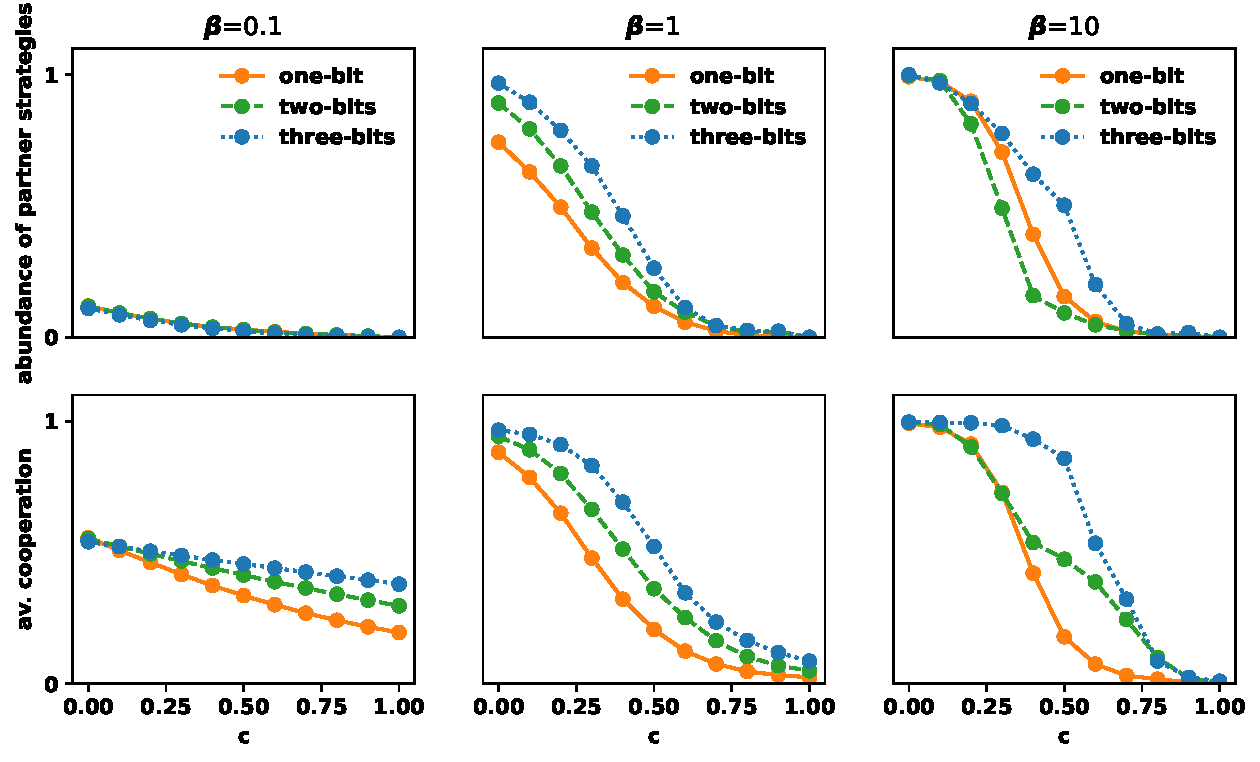
\includegraphics[width=\textwidth]{figures/abundance_of_partner_strategies.pdf}
  \caption{The abundance of partner strategies for $n=1,2,3$ and $b=1, c=0.5$.}
\end{figure}

\begin{figure}[!htbp]
  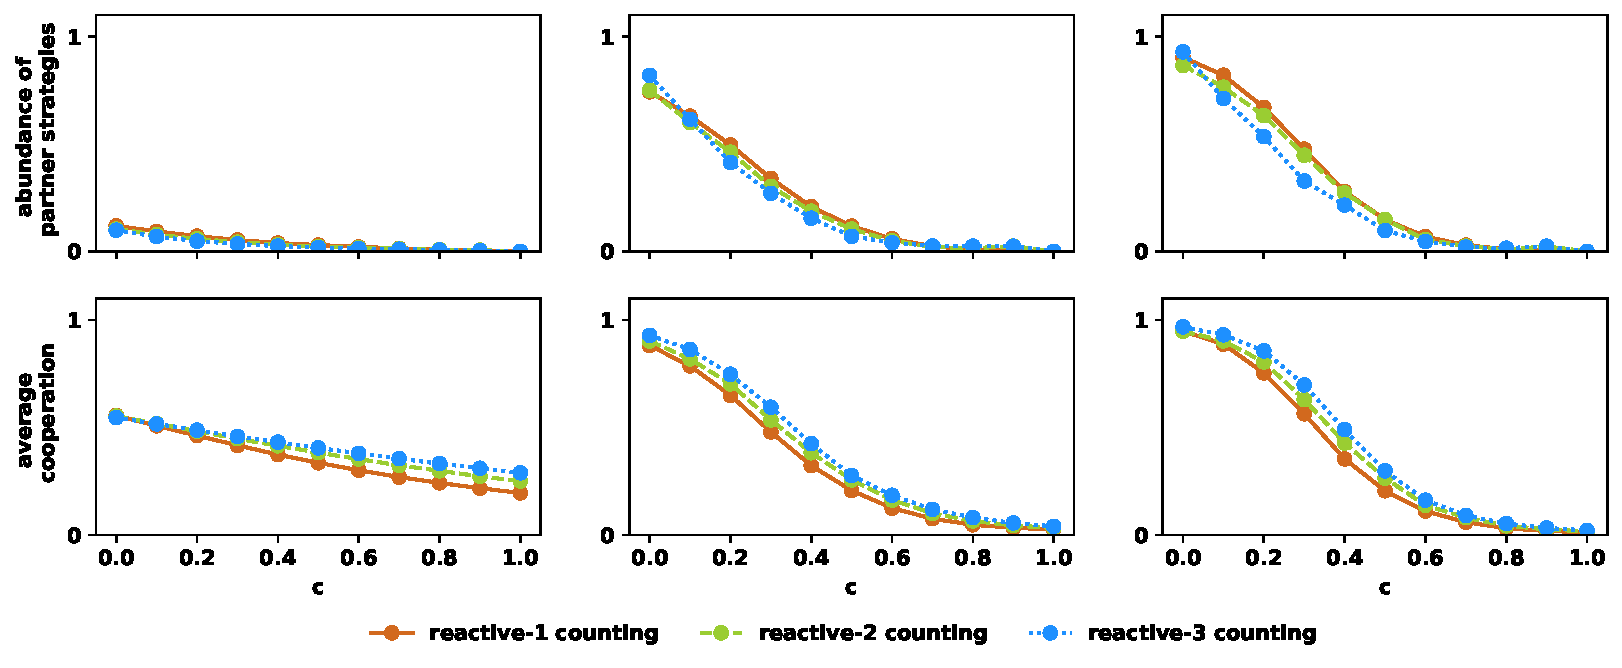
\includegraphics[width=\textwidth]{figures/abundance_of_partner_counting_strategies.pdf}
  \caption{The abundance of partner counting strategies for $n=1,2,3$ and $b=1, c=0.5$.}
\end{figure}

\begin{figure}[!htbp]
  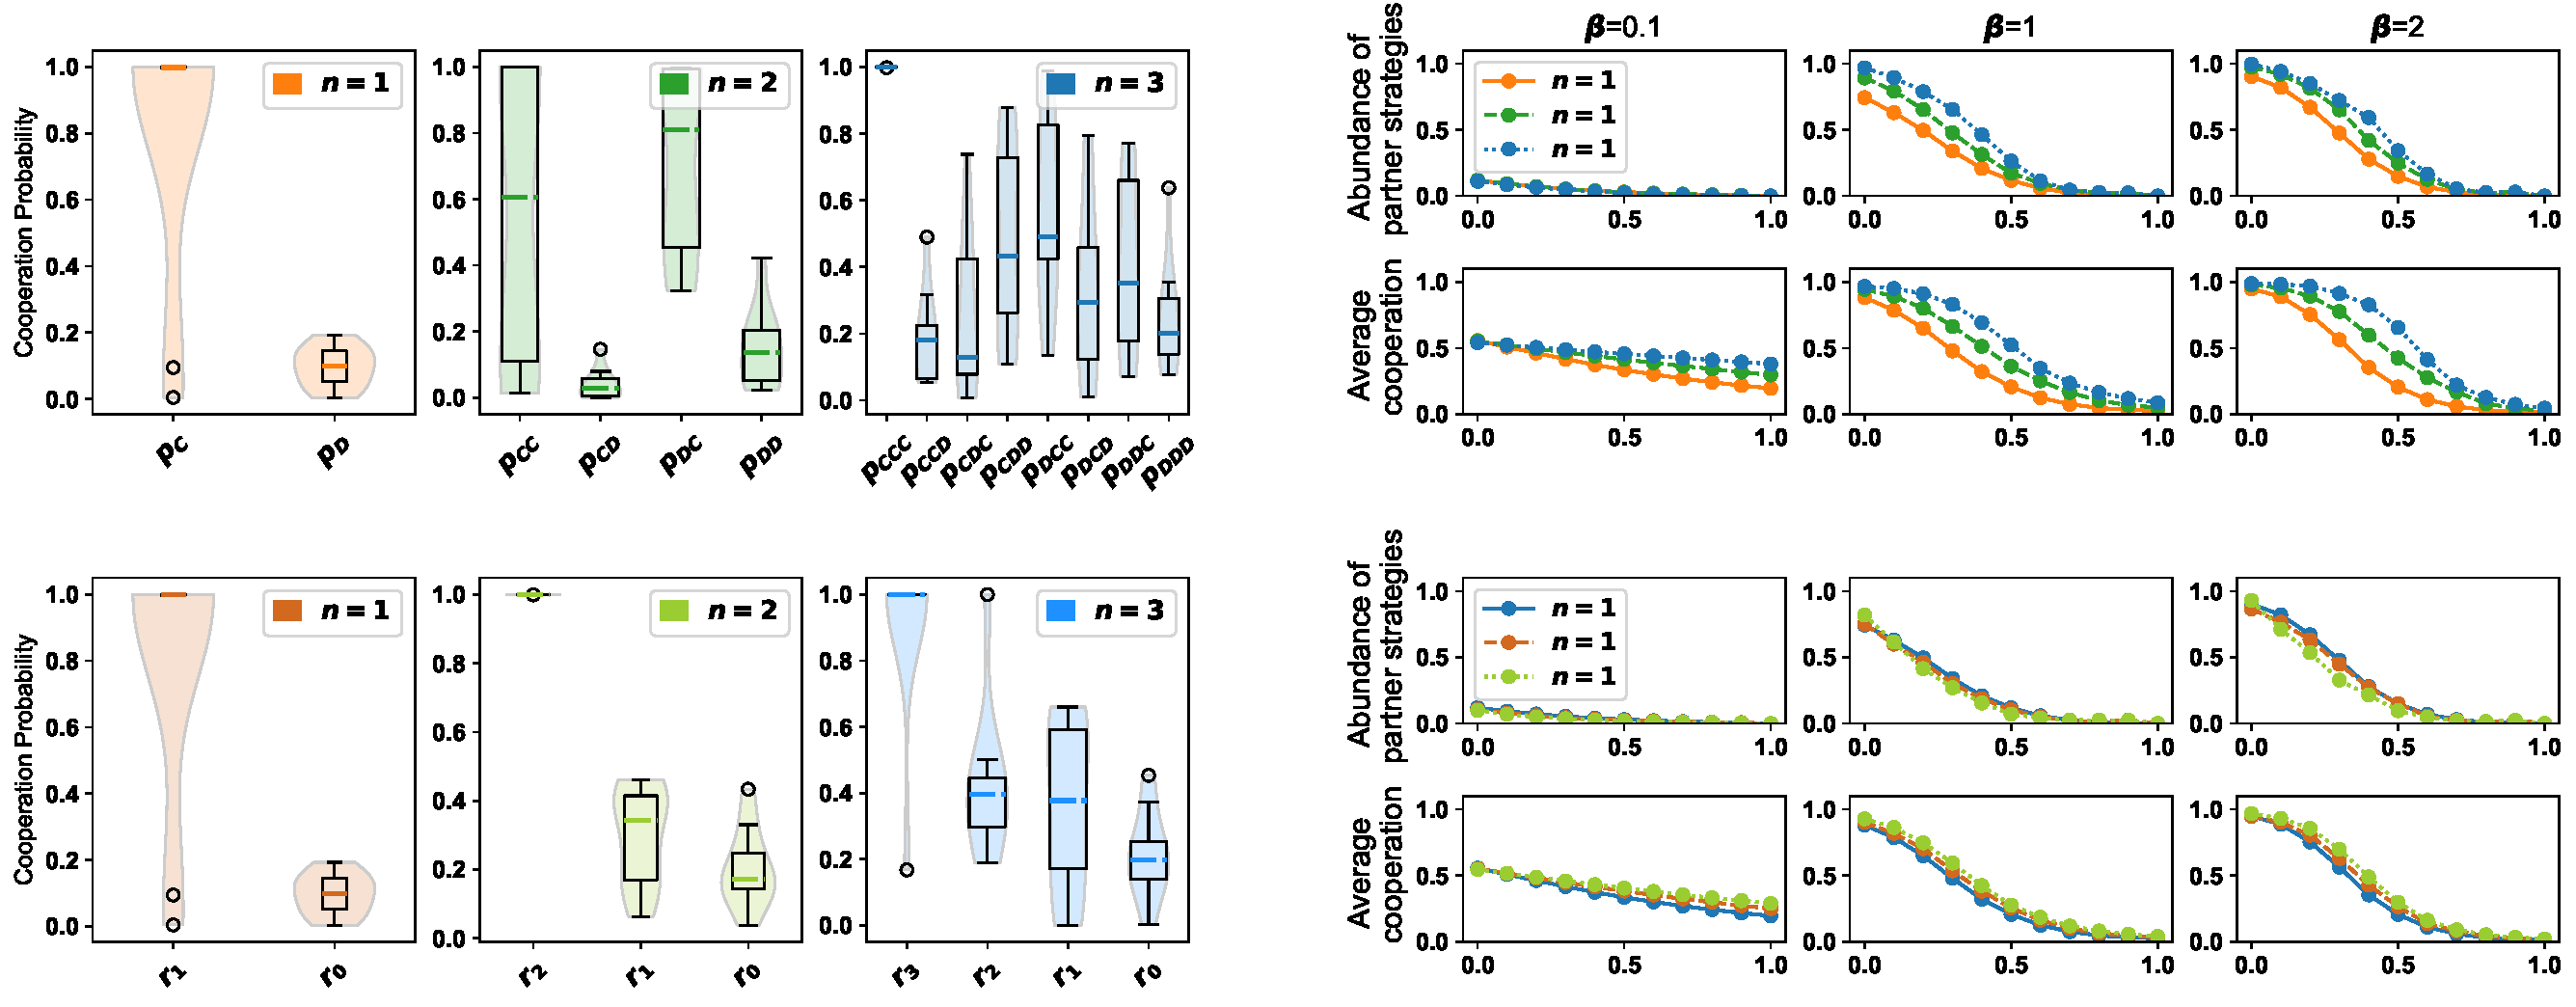
\includegraphics[width=\textwidth]{figures/abundant_strategies.pdf}
  \caption{The most abundant reactive-$n$ strategies for $n=1,2,3$ and $b=1, c=0.5, \beta=1$.}
\end{figure}

\begin{figure}[!htbp]
  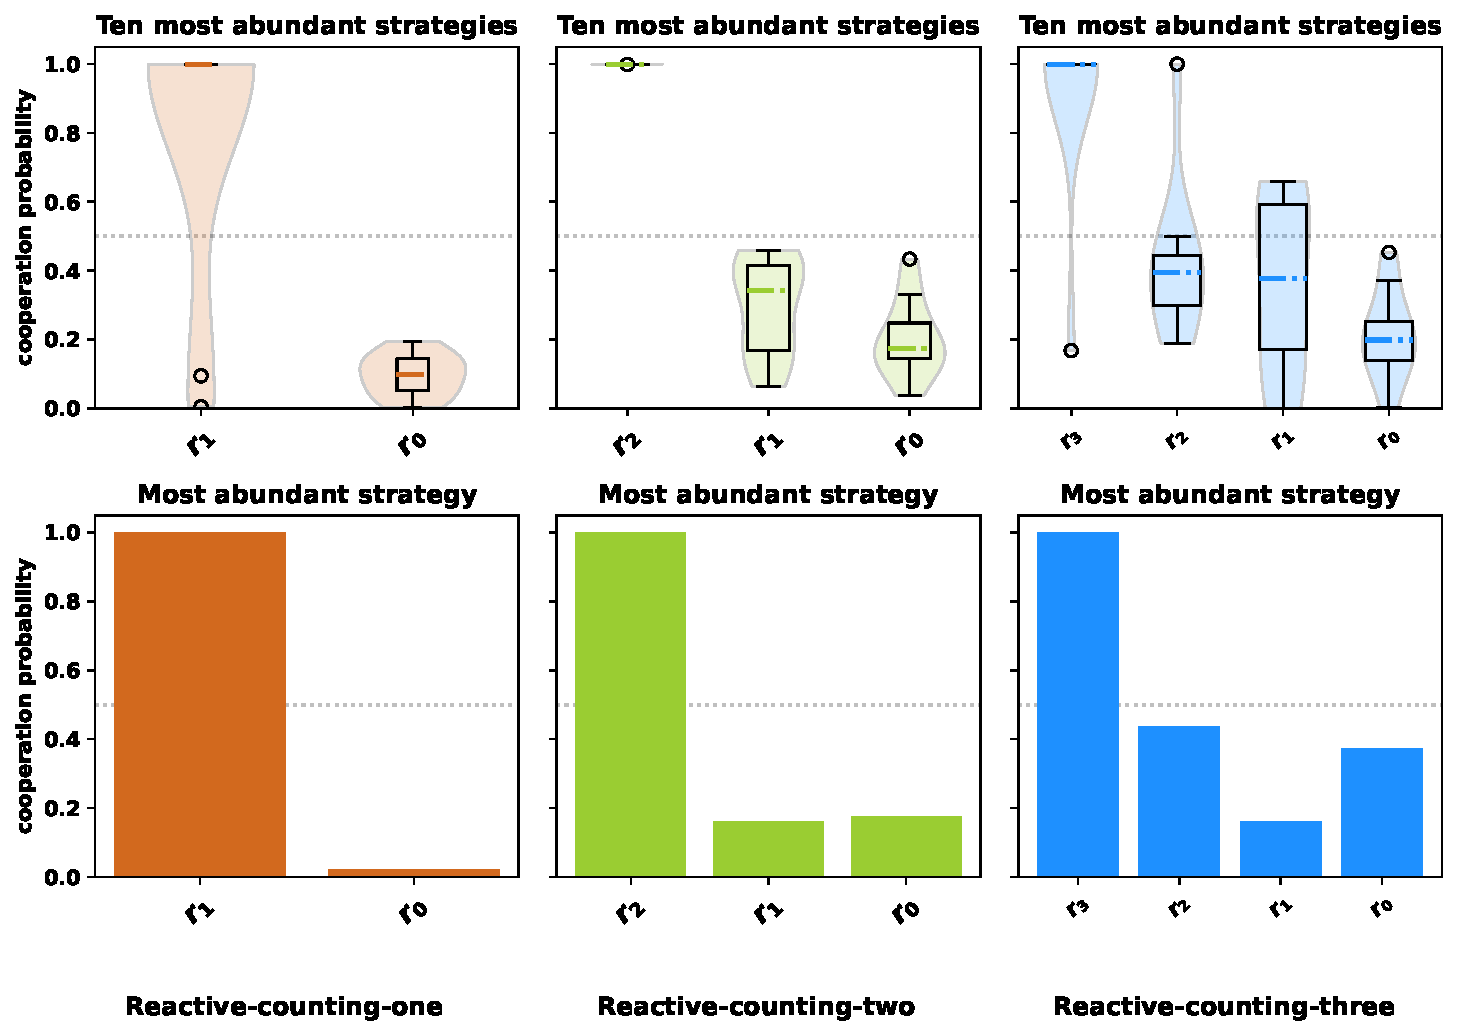
\includegraphics[width=\textwidth]{figures/abundant_strategies_counting.pdf}
  \caption{The most abundant reactive-counting-$n$ strategies for $n=1,2,3$ and $b=1, c=0.5, \beta=1$.}
\end{figure}

% \begin{figure}
%   \includegraphics[options]{fig}
% \end{figure}

~\\
\bibliography{bibliography.bib}

\end{document}